\documentclass{article}
\usepackage[utf8]{inputenc}
\usepackage{fancyhdr}
\usepackage{lastpage}
\usepackage{amsfonts}
\usepackage{amsmath}
\usepackage{amssymb}
\usepackage{bm}
\usepackage{bbm}
\usepackage{tikz}

\usetikzlibrary{shapes}
\usetikzlibrary{automata, positioning, arrows}

\usepackage[shortlabels]{enumitem}
\usepackage[noabbrev, capitalise]{cleveref}

\usepackage{geometry}
 \geometry{
 a4paper,
 top=20mm,
 bottom=25mm,
 left=25mm,
 right=25mm,
 }

% define your IDs here:
\newcommand{\firststudentid}{123456789}
\newcommand{\secondstudentid}{987654321}

\pagestyle{fancy}
\fancyhf{}
\rhead{Written Solution for Assignment 1}
\chead{\firststudentid \qquad \secondstudentid}
\lhead{Natural Language Processing}
\rfoot{Page \thepage \hspace{1pt} of \pageref{LastPage}}
\renewcommand{\footrulewidth}{1pt}
 
\setlength{\parindent}{0pt}
\setlength{\parskip}{1em}
\renewcommand{\baselinestretch}{1.25}

\renewcommand{\thesubsection}{\thesection.\alph{subsection}}
\renewcommand{\thesubsubsection}{\thesubsection.\roman{subsubsection}}

\begin{document}

\section{Word-Level Neural Bigram Language Model}
\subsection{Gradient of Softmax + CE}
\subparagraph{•}
Denote SCE - Softmax Cross Entropy function:\\
$SCE(\theta, y) = CE(\hat{y}, y) = CE(softmax(\theta), y) \\$
$= -\sum_{i} y_i log(\hat{y}_i)\\$
$if \ k \ - \ true \ label:\\$
$= - log(\hat{y}_i) = -log(softmax(\theta)_k) = -log(\frac{exp(\theta_k)}{\sum_{j}exp(\theta_j)})\\$
$= log(\sum_{j}exp(\theta_j))-\theta_k\\$
$\Longrightarrow SCE(\theta, y) = log(\sum_{j}exp(\theta_j))-\theta_k\\$

\subparagraph{•}
Now let's calculate it's derivative with respect to some $\theta_i:\\$
$\frac{\delta SCE}{\delta \theta_i} = \frac{log(\sum_{j}exp(\theta_j))}{\delta \theta_i} -\frac{\delta \theta_k}{\delta \theta_i}\\$
$\downarrow \\$
$denote: \ f \ = \sum_{j}exp(\theta_j)\\ $
$\downarrow \\$
$\frac{log(\sum_{j}exp(\theta_j))}{\delta \theta_i} -\frac{\delta \theta_k}{\delta \theta_i}\\$
$= \frac{log(f)}{\delta f}\frac{\delta f}{\delta \theta_i} -\frac{\delta \theta_k}{\delta \theta_i}\\$
$= \frac{1}{f} \sum_{j} \frac{exp(\theta_j)}{exp(\theta_i)} -\frac{\delta \theta_k}{\delta \theta_i}\\$
$= \frac{1}{f} exp(\theta_i) -\frac{\delta \theta_k}{\delta \theta_i}\\$
$= \frac{exp(\theta_i)}{\sum_{j} exp(\theta_j)}-\frac{\delta \theta_k}{\delta \theta_i}\\$
$= \frac{exp(\theta_i)}{\sum_{j} exp(\theta_j)} - \mathbbm{1}(i=k)\\$
$= softmax(\theta)_i - \mathbbm{1}(i=k)\\$
$\Longrightarrow \nabla_\theta SCE = softmax(\theta) - y = \hat{y}-y\\$ 

\subparagraph{•}
Basically the gradient of this function is prediction softmax vector minus true label one-hot vector.

\subsection{Gradients of NN}
\subparagraph{•}
In this section we use:\\
$h=\sigma(x W_1 + b_1) \\$
$\theta = h W_2 + b_2 \\$
$\hat{y}= softmax(\theta) \\$
$CE(y,\hat{y}) = -\sum_{i} y_i log(\hat{y}_i)\\$
$\nabla_\theta SCE = \hat{y}-y$

\subparagraph{•}
Also notice that Jacobian matrix of a vector function sigmoid is:\\
$da(\sigma (a))=diag(\sigma' (a))= \begin{bmatrix}
\sigma' (a_1) & 0 & 0 & 0\\
0 & \sigma' (a_2) & 0 & 0\\
0 & 0 & \sigma' (a_i) & 0\\
0 & 0 & 0 & \sigma' (a_n) 
\end{bmatrix} \ ; \ \sigma' (a_i)=\sigma(a_i)(1-\sigma(a_i))$

\subparagraph{•}
Let's write a formula for each gradient using differentials:

\subparagraph{•}
$dx(SCE)=dx(SCE(hW_2+b_2)) \\$
$= \nabla_\theta SCE \ dx(hW_2+b_2) \\$
$= \nabla_\theta SCE \ dx(hW_2) \\$
$= \nabla_\theta SCE \ W_2^T \ dx(h) \\$
$= \nabla_\theta SCE \ W_2^T \ dx(\sigma (xW_1+b_1)) \\$
$= \nabla_\theta SCE \ W_2^T \ diag(\sigma' (xW_1+b_1)) \ dx(xW_1+b_1) \\$
$= \nabla_\theta SCE \ W_2^T \ diag(\sigma' (xW_1+b_1)) \ W_1^T \ dx \\$
$\Longrightarrow \nabla_x SCE = \nabla_\theta SCE \ W_2^T \ diag(\sigma' (xW_1+b_1)) \ W_1^T \\$
$\Longrightarrow \nabla_x SCE = (\hat{y}-y) \ W_2^T \ diag(\sigma' (xW_1+b_1)) \ W_1^T$

This formula won't work for batched data, but we can write it in the more generic way using Hadamard product, i.e. elementwise multiplication - $\circ$ :

$\Longrightarrow \nabla_x SCE = \{ (\hat{y}-y) \ W_2^T \ \circ\ \sigma' (xW_1+b_1)\} \ W_1^T$

\subparagraph{•}
Let's sanity check it's dimentions:\\
$x - 2 \times 10 \ $ (batch of two vectors)\\
$W_1 - 10 \times 7 \\$
$b_1 - 1 \times 7 \\$
$\sigma(xW_1+b_1) - 2 \times 7 $ (bias is broadcasted)\\
$\sigma'(xW_1+b_1) - 2 \times 7 $ (bias is broadcasted)\\
$W_2 - 7 \times 5 \\$
$b_2 - 1 \times 5 \\$
$y - 2 \times 5 $ (batch of two vectors)\\

$\Longrightarrow \nabla_x SCE = \{ (\hat{y}-y) \ W_2^T \ \circ\ \sigma' (xW_1+b_1)\} \ W_1^T\\$
$\Longrightarrow \ 2 \ \times \ 10 \  = \{ (2 \times 5) \ (5 \times 7) \ \circ\ (2 \times 7)\} \ (7 \times 10)$

All dimensions match.

\subparagraph{•}
$dW_1(SCE)=dW_1(SCE(hW_2+b_2)) \\$
$= \nabla_\theta SCE \ dW_1(hW_2+b_2) \\$
$= \nabla_\theta SCE \ dW_1(hW_2) \\$
$= \nabla_\theta SCE \ W_2^T \ dW_1(h) \\$
$= \nabla_\theta SCE \ W_2^T \ dW_1(\sigma (xW_1+b_1)) \\$
$= \nabla_\theta SCE \ W_2^T \ diag(\sigma' (xW_1+b_1)) \ dW_1(xW_1+b_1) \\$
$= x^T \ \nabla_\theta SCE \ W_2^T \ diag(\sigma' (xW_1+b_1)) \ dW_1 \\$
$\Longrightarrow \nabla_{W_1} SCE = x^T \ \nabla_\theta SCE \ W_2^T \ diag(\sigma' (xW_1+b_1)) \\$
$\Longrightarrow \nabla_{W_1} SCE = x^T \ (\hat{y}-y) \ W_2^T \ diag(\sigma' (xW_1+b_1))$

Same trick with Hadamard product, i.e. elementwise multiplication - $\circ$ :\\
$\Longrightarrow \nabla_{W_1} SCE = x^T \ \{ (\hat{y}-y) \ W_2^T \ \circ \ \sigma' (xW_1+b_1) \}$

\subparagraph{•}
$db_1(SCE)=db_1(SCE(hW_2+b_2)) \\$
$= \nabla_\theta SCE \ db_1(hW_2+b_2) \\$
$= \nabla_\theta SCE \ db_1(hW_2) \\$
$= \nabla_\theta SCE \ W_2^T \ db_1(h) \\$
$= \nabla_\theta SCE \ W_2^T \ db_1(\sigma (xW_1+b_1)) \\$
$= \nabla_\theta SCE \ W_2^T \ diag(\sigma' (xW_1+b_1)) \ db_1(xW_1+b_1) \\$
$= \nabla_\theta SCE \ W_2^T \ diag(\sigma' (xW_1+b_1)) \ 1 \ db_1 \\$
$\Longrightarrow \nabla_{b_1} SCE = \nabla_\theta SCE \ W_2^T \ diag(\sigma' (xW_1+b_1)) \\$
$\Longrightarrow \nabla_{b_1} SCE = (\hat{y}-y) \ W_2^T \ diag(\sigma' (xW_1+b_1))$

Same trick with Hadamard product, i.e. elementwise multiplication - $\circ$ :\\
$\Longrightarrow \nabla_{b_1} SCE \approx \{ (\hat{y}-y) \ W_2^T \} \ \circ \ \sigma' (xW_1+b_1)$

Notice that dims don't match, because bias was broadcasted. To match the dims, we sum the gradient along batch dimension.

$\Longrightarrow \nabla_{b_1} SCE = \sum_{batch=0}^N \{ \{ (\hat{y}-y) \ W_2^T \} \ \circ \ \sigma' (xW_1+b_1)\} _{batch}$

\subparagraph{•}
$dW_2(SCE)=dW_2(SCE(hW_2+b_2)) \\$
$= \nabla_\theta SCE \ dW_2(hW_2+b_2) \\$
$= \nabla_\theta SCE \ dW_2(hW_2) \\$
$= \nabla_\theta SCE \ h \ dW_2 \\$
$= \sigma (xW_1+b_1)^T \ \nabla_\theta SCE \ dW_2 \\$
$\Longrightarrow \nabla_{W_2} SCE = \sigma (xW_1+b_1)^T \ \nabla_\theta SCE \\$
$\Longrightarrow \nabla_{W_2} SCE = \sigma (xW_1+b_1)^T \ (\hat{y}-y)$

\subparagraph{•}
$db_2(SCE)=db_2(SCE(hW_2+b_2)) \\$
$= \nabla_\theta SCE \ db_2(hW_2+b_2) \\$
$= \nabla_\theta SCE \ 1 \ dW_2 \\$
$\Longrightarrow \nabla_{b_2} SCE = \nabla_\theta SCE \\$
$\Longrightarrow \nabla_{b_2} SCE \approx (\hat{y}-y) $

Adjust dims:\\
$\Longrightarrow \nabla_{b_2} SCE = \sum_{batch=0}^N (\hat{y}-y)_{batch} $

\subsection{}

\subsection{Perplexity}
Dev perplexity : 112.889

\section*{Section 2 - Theoretical Inquiry of a Simple RNN Language Model}

\begin{itemize}
    \item[(a)]
    Some notation: Denote the elements of the matrices $\mathbf{H}, \mathbf{I}, \mathbf{U}, \mathbf{L}$ by $H_{ij}$, $I_{ij}$, $U_{ij}$, $L_{ij}$. Let $\delta_{ij} = \begin{cases} 1 & \text{if } i=j \\ 0 & \text{otherwise}\end{cases}$ (Kroenecker delta). Also note that $\mathbf{L}_{\mathbf{x}^(t)} = \mathbf{e}^{(t)}$
    
    We will also omit $\left. \right|_{(t)}$ for notational simplicity but it is assumed when needed.
    
    
    Let $\boldsymbol{\theta}^{(t)}_1 = \mathbf{h}^{(t-1)}\mathbf{H} + \mathbf{e}^{(t)}\mathbf{I} + \mathbf{b}_1$  (logit vector), and denote its $k$-th element by $\theta_{1,k}^{(t)}$. Calculate its derivatives with respect to the various model parameters:
    
    \begin{align*}
        \frac{\partial \theta^{(t)}_{1, k}}{\partial H_{ij}} &= \frac{\partial}{\partial H_{ij}} \left(\sum_{\ell}h^{(t-1)}_\ell H_{\ell k}\right) = h_i^{(t-1)} \delta_{jk}\\
        \frac{\partial \theta^{(t)}_{1,k}}{\partial I_{ij}} &= \frac{\partial}{\partial I_{ij}} \left(\sum_{\ell}e^{(t)}_\ell I_{\ell k}\right) = e_i^{(t)} \delta_{jk}\\
        \frac{\partial \theta^{(t)}_{1,k}}{\partial b_{1,i}} &= \delta_{ik}\\
        \frac{\partial \theta_{1,k}^{(t)}}{e^{(t)}_i} &= I_{ik}\\
        \frac{\partial \theta^{(t)}_{1, k}}{\partial h_i^{(t-1)}} &= \frac{\partial}{\partial h_i^{(t-1)}} \left(\sum_{\ell}h^{(t-1)}_\ell H_{\ell k}\right) = H_{ik}\\
    \end{align*}
    
    We have $\mathbf{h}^{(t)} = \sigma(\boldsymbol{\theta}_1^{(t)})$. Defining $\boldsymbol{\theta}^{(t)}_2 = \mathbf{h}^{(t)}\mathbf{U} + \mathbf{b}_2$ (logit vector) and denoting its $k$-th element by $\theta^{(t)}_{2,k}$, by the chain rule we have
    
    \begin{align*}
        \frac{\partial \theta_{2,k}^{(t)}}{\partial H_{ij}} &= \frac{\partial}{\partial H_{ij}} \left( \sum_\ell h_\ell^{(t)}U_{\ell k} \right) \\
        &= \sum_\ell \frac{\partial h_\ell^{(t)}}{\partial H_{ij}}U_{\ell k}
    \end{align*}
    
    \begin{align*}
        &= \sum_\ell \sigma'(\theta_{1, \ell}^{(t)})\frac{\partial \theta_{1, \ell}^{(t)}}{\partial H_{ij}} U_{\ell k} \\
        &= \sum_\ell \sigma'(\theta_{1, \ell}^{(t)}) h_{i}^{(t-1)}\delta_{j\ell} U_{\ell k} \\
        &= \sigma'(\theta_{1, k}^{(t)}) h_{i}^{(t-1)} U_{j k} \\
        \\
        \frac{\partial \theta_{2,k}^{(t)}}{\partial I_{ij}} &= \sum_\ell \sigma'(\theta_{1, \ell}^{(t)})\frac{\partial \theta_{1, \ell}^{(t)}}{\partial I_{ij}} U_{\ell k} \\
        &= \sum_\ell \sigma'(\theta_{1, \ell}^{(t)}) e_i^{(t)}\delta_{j\ell} U_{\ell k} \\
        &= \sigma'(\theta_{1, j}^{(t)}) e_i^{(t)} U_{j k} \\
        \\
        \frac{\partial \theta_{2,k}^{(t)}}{\partial b_{1,i}} &= \sum_\ell \sigma'(\theta_{1, \ell}^{(t)})\frac{\partial \theta_{1, \ell}^{(t)}}{\partial b_{1,i}} U_{\ell k} \\
        &= \sum_\ell \sigma'(\theta_{1, \ell}^{(t)}) \delta_{i\ell} U_{\ell k} \\
        &= \sigma'(\theta_{1, i}^{(t)}) U_{i k} \\
        \\
        \frac{\partial \theta_{2,k}^{(t)}}{\partial e_i^{(t)}} &= \sum_\ell \sigma'(\theta_{1, \ell}^{(t)})\frac{\partial \theta_{1, \ell}^{(t)}}{\partial e_i^{(t)}} U_{\ell k}\\
        &= \sum_\ell \sigma'(\theta_{1, \ell}^{(t)}) I_{i \ell} U_{\ell k}\\
        \\
        \frac{\partial \theta_{2,k}^{(t)}}{b_{2,i}} &= \delta_{ik}
        \\
        \frac{\partial \theta_{2,k}^{(t)}}{U_{ij}} &= \frac{\partial}{\partial U_{ij}} \left( \sum_\ell h_\ell^{(t)}U_{\ell k} \right) \\
        &= h_i^{(t)}\delta_{jk}\\
    \end{align*}
    
    \begin{align*}
        \frac{\partial \theta_{2,k}^{(t)}}{h_i^{(t-1)}} &= \sum_\ell \sigma'(\theta_{1, \ell}^{(t)})\frac{\partial \theta_{1, \ell}^{(t)}}{\partial h_i^{(t-1)}} U_{\ell k} \\
        &= \sum_\ell \sigma'(\theta_{1, \ell}^{(t)}) H_{i\ell} U_{\ell k}
    \end{align*}
    
    Recall that $\sigma'(t) = \sigma(t)(1-\sigma(t))$.
    
    Now since $J^{(t)} = \text{CE}(\mathbf{y}^{(t)}, \hat{\mathbf{y}}^{(t)})$ and $\hat{\mathbf{y}}^{(t)} = \text{softmax}(\boldsymbol{\theta}_2^{(t)})$, by the result from problem 1a $\nabla_{\boldsymbol{\theta}_2^{(t)}} J^{(t)} = \mathbf{y}^{(t)} - \text{softmax}(\boldsymbol{\theta}_2^{(t)})$, i.e. $\frac{\partial J^{(t)}}{\theta_{2, k}^{(t)}} = y_k^{(t)} - \text{softmax}(\boldsymbol{\theta}_2^{(t)})_k$. Therefore we can calculate the derivatives of $J$ with respect to the various parameters by the chain rule:
    
    \begin{align*}
        \frac{\partial J^{(t)}}{\partial H_{ij}} &= \sum_k \frac{\partial J^{(t)}}{\partial \theta_{2, k}^{(t)}} \frac{\partial \theta_{2, k}^{(t)}}{\partial H_{ij}}\\
        &= \sum_k (y_k^{(t)} - \text{softmax}(\boldsymbol{\theta}_2^{(t)})_k) \sigma'(\theta_{1, k}^{(t)}) h_{i}^{(t-1)} U_{j k}\\
        \frac{\partial J^{(t)}}{\partial \bold{H}} &= \mathbf{h}^{(t-1)T}(\mathbf{y}^{(t)}-\text{softmax}(\boldsymbol{\theta}_2^{(t)}))\boldsymbol{\Sigma}(\boldsymbol{\theta}_1^{(t)}) \mathbf{U}^T
    \end{align*}
    
    where we define $\boldsymbol{\Sigma}(\mathbf{v})$ as in problem 1a to be the diagonal matrix with $i$-th diagonal element $\sigma'(v_i)=\sigma(v_i)(1-\sigma(v_i))$.
    
    \begin{align*}
        \frac{\partial J^{(t)}}{\partial I_{ij}} &= \sum_k \frac{\partial J^{(t)}}{\partial \theta_{2, k}^{(t)}} \frac{\partial \theta_{2, k}^{(t)}}{\partial I_{ij}}\\
        &= \sum_k (y_k^{(t)} - \text{softmax}(\boldsymbol{\theta}_2^{(t)})_k) \sigma'(\theta_{1, j}^{(t)}) e_i^{(t)} U_{j k}\\
        \frac{\partial J^{(t)}}{\partial \mathbf{I}} &= \mathbf{e}^{(t) T}(\mathbf{y}^{(t)}-\text{softmax}(\boldsymbol{\theta}_2^{(t)})) \mathbf{U}^T \boldsymbol{\Sigma}(\boldsymbol{\theta}_1^{(t)})\\
        \\
        \frac{\partial J^{(t)}}{\partial b_{1,i}} &= \sum_k \frac{\partial J^{(t)}}{\partial \theta_{2, k}^{(t)}} \frac{\partial \theta_{2, k}^{(t)}}{\partial b_{1,i}}\\
        &= \sum_k (y_k^{(t)} - \text{softmax}(\boldsymbol{\theta}_2^{(t)})_k) \sigma'(\theta_{1, i}^{(t)}) U_{ik}\\
        \frac{\partial J^{(t)}}{\partial \mathbf{b}_{1}} &= (\mathbf{y}^{(t)}-\text{softmax}(\boldsymbol{\theta}_2^{(t)})) \mathbf{U}^T \boldsymbol{\Sigma}(\boldsymbol{\theta}_1^{(t)}) \\
        \\
        \frac{\partial J^{(t)}}{\partial e_i^{(t)}} &= \sum_k \frac{\partial J^{(t)}}{\partial \theta_{2, k}^{(t)}} \frac{\partial \theta_{2, k}^{(t)}}{\partial e_i^{(t)}}\\
        &= \sum_k (y_k^{(t)} - \text{softmax}(\boldsymbol{\theta}_2^{(t)})_k) \sum_\ell \sigma'(\theta_{1, \ell}^{(t)})I_{i \ell}U_{\ell k}\\
        \frac{\partial J^{(t)}}{\partial \mathbf{L}_{\mathbf{x}^{(t)}}} &= \frac{\partial J^{(t)}}{\partial \mathbf{e}^{(t)}} = (\mathbf{y}^{(t)}-\text{softmax}(\boldsymbol{\theta}_2^{(t)})) \mathbf{U}^T \boldsymbol{\Sigma}(\boldsymbol{\theta}_1^{(t)})\mathbf{I}^T\\
    \end{align*}
    
    \begin{align*}
        \frac{\partial J^{(t)}}{\partial b_{2, i}} &= \sum_k \frac{\partial J^{(t)}}{\partial \theta_{2, k}^{(t)}} \frac{\partial \theta_{2, k}^{(t)}}{\partial b_{2,i}}\\
        &= \sum_k (y_k^{(t)} - \text{softmax}(\boldsymbol{\theta}_2^{(t)})_k) \delta_{ik}\\
        &= (y_i^{(t)} - \text{softmax}(\boldsymbol{\theta}_2^{(t)})_i)\\
        \frac{\partial J^{(t)}}{\partial \mathbf{b}_2} &= \mathbf{y}^{(t)} - \text{softmax}(\boldsymbol{\theta}_2^{(t)})\\
        \\
        \frac{\partial J^{(t)}}{\partial U_{ij}} &= \sum_k \frac{\partial J^{(t)}}{\partial \theta_{2, k}^{(t)}} \frac{\partial \theta_{2, k}^{(t)}}{\partial U_{ij}}\\
        &= \sum_k (y_k^{(t)} - \text{softmax}(\boldsymbol{\theta}_2^{(t)})_k) h_i^{(t)}\delta_{jk}\\
        &= (y_j^{(t)} - \text{softmax}(\boldsymbol{\theta}_2^{(t)})_j) h_i^{(t)} \\
        \frac{\partial J^{(t)}}{\partial \mathbf{U}} &= \mathbf{h}^{(t)T} (\mathbf{y}^{(t)} - \text{softmax}(\boldsymbol{\theta}_2^{(t)}))\\
        \\
        \frac{\partial J^{(t)}}{\partial h_i^{(t-1)}} &= \sum_k \frac{\partial J^{(t)}}{\partial \theta_{2, k}^{(t)}} \frac{\partial \theta_{2, k}^{(t)}}{\partial h_i^{(t-1)}}\\
        &= \sum_k (y_k^{(t)} - \text{softmax}(\boldsymbol{\theta}_2^{(t)})_k) \sum_\ell \sigma'(\theta_{1, \ell}^{(t)}) H_{i\ell} U_{\ell k}\\
        \frac{\partial J^{(t)}}{\partial \mathbf{h}^{(t-1)}} &= (\mathbf{y}^{(t)}-\text{softmax}(\boldsymbol{\theta}_2^{(t)})) \mathbf{U}^T \boldsymbol{\Sigma}(\boldsymbol{\theta}_1^{(t)})\mathbf{H}^T
    \end{align*}
    
    \item[(b)]
    
    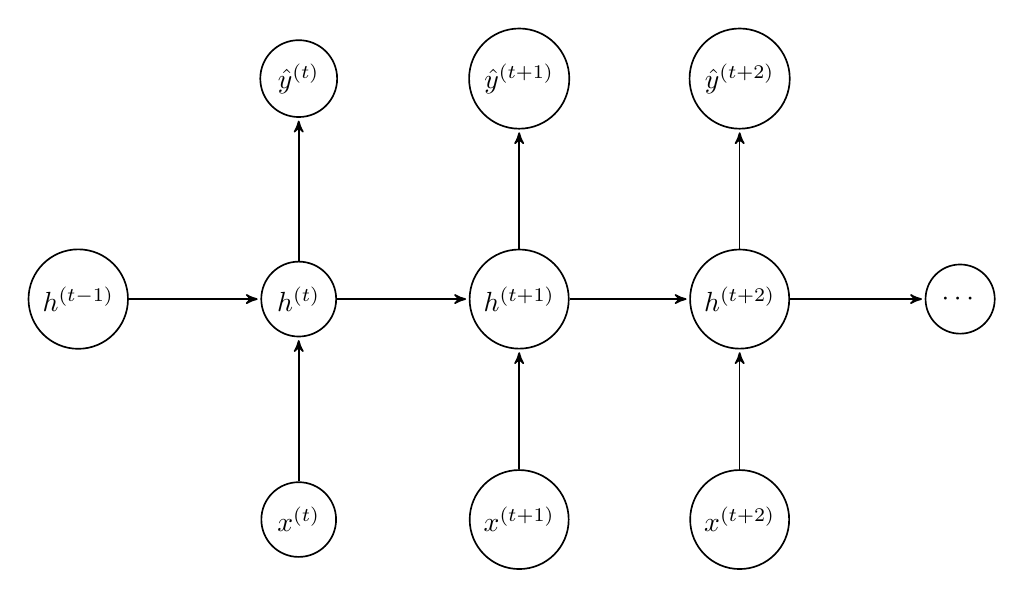
\begin{tikzpicture}[->,>=stealth',shorten >=1pt,auto,node distance=2.8cm, semithick]
    
    \node[state] (neg) {$h^{(t-1)}$};
    \node[state, right of=neg] (ht0) {$h^{(t)}$};
    \node[state, right of=ht0] (ht1) {$h^{(t+1)}$};
    \node[state, right of=ht1] (ht2) {$h^{(t+2)}$};
    \node[state, right of=ht2] (pos) {$\cdots$};
    
    \node[state, below of=ht0] (in0) {$x^{(t)}$};
    \node[state, below of=ht1] (in1) {$x^{(t+1)}$};
    \node[state, below of=ht2] (in2) {$x^{(t+2)}$};
    
    \node[state, above of=ht0] (out0) {$\hat{y}^{(t)}$};
    \node[state, above of=ht1] (out1) {$\hat{y}^{(t+1)}$};
    \node[state, above of=ht2] (out2) {$\hat{y}^{(t+2)}$};
    \draw
            (neg) edge (ht0)
            (ht0) edge (ht1)
            (ht1) edge (ht2)
            (ht2) edge (pos)
            
            (in0) edge (ht0)
            (in1) edge (ht1)
            (in2) edge (ht2)
            
            (ht0) edge (out0)
            (ht1) edge (out1)
            (ht2) edge (out2)
            ;
    \end{tikzpicture}
    
    
    First we calculate the following auxiliary quantities, using all the notation and results from part (a) above:
    
    \begin{align*}
        \frac{\partial J^{(t)}}{\partial \boldsymbol{\theta}_2^{(t)}} &= \mathbf{y}^{(t)} - \hat{\mathbf{y}}^{(t)} \\
        \frac{\partial J^{(t)}}{\partial h^{(t)}_i} &= \sum_j \frac{\partial J^{(t)}}{\partial \theta_{2,j}^{(t)}}\frac{\partial \theta_{2, j}^{(t)}}{\partial h^{(t)}_i}\\
        &= \sum_j (y^{(t)}_j - \hat{y}^{(t)}_j) \frac{\partial \theta_{2, j}^{(t)}}{\partial h^{(t)}_i} \\
        &= \sum_j (y^{(t)}_j - \hat{y}^{(t)}_j) \frac{\partial}{\partial h^{(t)}_i} (\sum_k h^{(t)}_k U_{kj} + b_{2, j}) \\
        &= \sum_j (y^{(t)}_j - \hat{y}^{(t)}_j) U_{ij} \\
        \frac{\partial J^{(t)}}{\partial \mathbf{h}^{(t)}} &= (\mathbf{y}^{(t)} - \hat{\mathbf{y}}^{(t)}) \mathbf{U}^T \\
        \frac{\partial J^{(t)}}{\partial \theta_{1, i}^{(t)}} &= \sum_j \frac{\partial J^{(t)}}{\partial h^{(t)}_j} \frac{\partial h^{(t)}_j}{\partial \theta_{1, i}^{(t)}} \\
        &= \sum_{j,k} (y^{(t)}_k - \hat{y}^{(t)}_k) U_{jk} \frac{\partial h^{(t)}_j}{\partial \theta_{1, i}^{(t)}} \\
        &= \sum_{j,k} (y^{(t)}_k - \hat{y}^{(t)}_k) U_{jk} \frac{\partial}{\partial \theta_{1, i}^{(t)}} \sigma(\theta_{1, j}^{(t)}) \\
        &= \sum_{j,k} (y^{(t)}_k - \hat{y}^{(t)}_k) U_{jk} \delta_{ij} \sigma'(\theta_{1, i}^{(t)}) \\
        &= \sum_{k} (y^{(t)}_k - \hat{y}^{(t)}_k) U_{ik} \sigma'(\theta_{1, i}^{(t)}) \\
        \frac{\partial J^{(t)}}{\partial \boldsymbol{\theta}_1^{(t)}} &= (\mathbf{y}^{(t)} - \hat{\mathbf{y}}^{(t)}) \mathbf{U}^T \boldsymbol{\Sigma}(\boldsymbol{\theta}_1^{(t)})
    \end{align*}
    \begin{align*}
        \frac{\partial h^{(t)}_i}{\partial e^{(t)}_j} &= \frac{\partial}{\partial e^{(t)}_j} \sigma(\sum_k h^{(t-1)}_k H_{ki} + \sum_k e^{(t)}_k I_{ki} + b_{1, i}) \\
        &= I_{ji} \sigma'(\sum_kh^{(t-1)}_k H_{ki} + \sum_k e^{(t)}_k I_{ki} + b_{1, i}) \\
        &= I_{ji} \sigma'(\theta^{(t)}_{1, i}) \\
        \frac{\partial h^{(t)}_i}{\partial H_{jk}} &= \frac{\partial}{\partial H_{jk}} \sigma(\sum_\ell h^{(t-1)}_\ell H_{\ell i} + \sum_\ell e^{(t)}_\ell I_{\ell i} + b_{1, i}) \\
        &= h_j^{(t-1)}\delta_{ik} \sigma'(\theta_{1, i}^{(t)}) \\
        \frac{\partial h^{(t)}_i}{\partial I_{jk}} &= \frac{\partial}{\partial I_{jk}} \sigma(\sum_\ell h^{(t-1)}_\ell H_{\ell i} + \sum_\ell e^{(t)}_\ell I_{\ell i} + b_{1, i}) \\
        &= e_j^{(t)}\delta_{ik} \sigma'(\theta_{1, i}^{(t)}) \\
        \frac{\partial h^{(t)}_i}{\partial b_{1,j}} &= \frac{\partial}{\partial b_{1,j}} \sigma(\sum_\ell h^{(t-1)}_\ell H_{\ell i} + \sum_\ell e^{(t)}_\ell I_{\ell i} + b_{1, i}) \\
        &= \delta_{ij} \sigma'(\theta_{1, i}^{(t)})
    \end{align*}
    
    
    Now we can calculate the desired quantities:
    
    \begin{align*}
        \frac{\partial J^{(t)}}{\partial L_{\mathbf{x}^{(t-1)}, k}} &= \frac{\partial J^{(t)}}{\partial e^{(t-1)}_k} = \sum_i \frac{\partial J^{(t)}}{\partial \theta_{1,i}^{(t)}} \frac{\partial \theta_{1,i}^{(t)}}{\partial e^{(t-1)}_k} \\
        &= \sum_{i,j} (y^{(t)}_j - \hat{y}^{(t)}_j) U_{ij} \sigma'(\theta_{1, i}^{(t)}) \frac{\partial \theta_{1,i}^{(t)}}{\partial e^{(t-1)}_k} \\
        &= \sum_{i,j} (y^{(t)}_j - \hat{y}^{(t)}_j) U_{ij} \sigma'(\theta_{1, i}^{(t)}) \frac{\partial}{\partial e^{(t-1)}_k} (\sum_\ell h^{(t-1)}_\ell H_{\ell i}) \\
        &= \sum_{i,j,\ell} (y^{(t)}_j - \hat{y}^{(t)}_j) U_{ij} \sigma'(\theta_{1, i}^{(t)}) H_{\ell i} \frac{\partial h^{(t-1)}_\ell}{\partial e^{(t-1)}_k} \\
        &= \sum_{i,j,\ell} (y^{(t)}_j - \hat{y}^{(t)}_j) U_{ij} \sigma'(\theta_{1, i}^{(t)}) H_{\ell i} I_{k\ell} \sigma'(\theta^{(t-1)}_{1, \ell}) \\
        \frac{\partial J^{(t)}}{\partial \mathbf{L}_{\mathbf{x}^{(t-1)}}} &= (\mathbf{y}^{(t)}-\hat{\mathbf{y}}^{(t)}_k) \mathbf{U}^T \boldsymbol{\Sigma}(\boldsymbol{\theta}_1^{(t)}) \mathbf{H}^T \boldsymbol{\Sigma}(\boldsymbol{\theta}_1^{(t-1)}) \mathbf{I}^T \\
        \left. \frac{\partial J^{(t)}}{\partial H_{mn}} \right|_{(t-1)} &= \sum_{i,j,\ell} (y^{(t)}_j - \hat{y}^{(t)}_j) U_{ij} \sigma'(\theta_{1, i}^{(t)}) H_{\ell i} \left.\frac{\partial h^{(t-1)}_\ell}{\partial H_{mn}}\right|_{(t-1)} \:\:\:\text{(by the same logic as above)}\\
        &= \sum_{i,j,\ell} (y^{(t)}_j - \hat{y}^{(t)}_j) U_{ij} \sigma'(\theta_{1, i}^{(t)}) H_{\ell i} h^{(t-2)}_m \delta_{\ell n} \sigma'(\theta^{(t-1)}_{1, \ell}) \\
        &= \sum_{i,j} (y^{(t)}_j - \hat{y}^{(t)}_j) U_{ij} \sigma'(\theta_{1, i}^{(t)}) H_{n i} h^{(t-2)}_m \sigma'(\theta^{(t-1)}_{1, n}) \\
        \left. \frac{\partial J^{(t)}}{\partial \mathbf{H}} \right|_{(t-1)} &= \mathbf{h}^{(t-2) T} (\mathbf{y}^{(t)}-\hat{\mathbf{y}}^{(t)}_k) \mathbf{U}^T \boldsymbol{\Sigma}(\boldsymbol{\theta}_1^{(t)}) \mathbf{H}^T \boldsymbol{\Sigma}(\boldsymbol{\theta}_1^{(t-1)}) \\
        \left. \frac{\partial J^{(t)}}{\partial I_{mn}} \right|_{(t-1)} &= \sum_{i,j,\ell} (y^{(t)}_j - \hat{y}^{(t)}_j) U_{ij} \sigma'(\theta_{1, i}^{(t)}) H_{\ell i} \left.\frac{\partial h^{(t-1)}_\ell}{\partial I_{mn}}\right|_{(t-1)} \:\:\:\text{(by the same logic as above)}\\
        &= \sum_{i,j,\ell} (y^{(t)}_j - \hat{y}^{(t)}_j) U_{ij} \sigma'(\theta_{1, i}^{(t)}) H_{\ell i} e^{(t-1)}_m \delta_{\ell n} \sigma'(\theta^{(t-1)}_{1, \ell}) \\
        &= \sum_{i,j} (y^{(t)}_j - \hat{y}^{(t)}_j) U_{ij} \sigma'(\theta_{1, i}^{(t)}) H_{n i} e^{(t-1)}_m \sigma'(\theta^{(t-1)}_{1, n}) \\
        \left. \frac{\partial J^{(t)}}{\partial \mathbf{I}} \right|_{(t-1)} &= \mathbf{e}^{(t-1) T} (\mathbf{y}^{(t)}-\hat{\mathbf{y}}^{(t)}_k) \mathbf{U}^T \boldsymbol{\Sigma}(\boldsymbol{\theta}_1^{(t)}) \mathbf{H}^T \boldsymbol{\Sigma}(\boldsymbol{\theta}_1^{(t-1)}) \\
    \end{align*}
    \begin{align*}
        \left. \frac{\partial J^{(t)}}{\partial b_{1,k}} \right|_{(t-1)} &= \sum_{i,j,\ell} (y^{(t)}_j - \hat{y}^{(t)}_j) U_{ij} \sigma'(\theta_{1, i}^{(t)}) H_{\ell i} \left.\frac{\partial h^{(t-1)}_\ell}{\partial b_{1,k}}\right|_{(t-1)} \\
        &= \sum_{i,j,\ell} (y^{(t)}_j - \hat{y}^{(t)}_j) U_{ij} \sigma'(\theta_{1, i}^{(t)}) H_{\ell i} \delta_{\ell k}\sigma'(\theta_{1, \ell}^{(t-1)}) \\
        &= \sum_{i,j} (y^{(t)}_j - \hat{y}^{(t)}_j) U_{ij} \sigma'(\theta_{1, i}^{(t)}) H_{k i} \sigma'(\theta_{1, k}^{(t-1)}) \\
        \left. \frac{\partial J^{(t)}}{\partial \mathbf{b}_1} \right|_{(t-1)} &= (\mathbf{y}^{(t)}-\hat{\mathbf{y}}^{(t)}_k) \mathbf{U}^T \boldsymbol{\Sigma}(\boldsymbol{\theta}_1^{(t)}) \mathbf{H}^T \boldsymbol{\Sigma}(\boldsymbol{\theta}_1^{(t-1)})
    \end{align*}
\end{itemize}

\section{GRU question}
\paragraph{Advantage}
Smaller discrete space - There are about 100 English-language characters in common usage if we include all punctuation marks. By contrast, a vocabulary is many thousands of words. For char-based model we need about 100 embeddings to represent all possible tokens.

\paragraph{Disadvantage}
Char-level models can generate unusual words. Word-level models can't generate mistyped words as these are not in their vocabulary. 

\section{Perplexity}

Write $p_i = p(s_i|s_1,\ldots,s_{i-1})$. Then for any $b > 0$,

$$b^{-\frac{1}{M}\sum_{i=1}^M \log_b p_i} = (b^{\sum_{i=1}^M \log_b p_i})^{-1/M} = (\prod_{i=1}^M b^{\log_b p_i})^{-1/M} = (\prod_{i=1}^M p_i)^{-1/M}$$

Therefore this expression has the same value for any such $b$, and in particular for $b=2$ and $b=e$ which are the two given expressions.


\end{document}